%\vspace*{40ex}
%
\section{Greedy Heuristic Distributions for Set Cover} \label{sec_cover}
\noindent
%\vspace*{-1ex} %%! DO NOT USE HERE!!

%https://www.amazon.com/s?k=models+of+my+life+by+herbert+simon 
%
%Here is the a snippet from the quote I was looking for:
%  “I think I invented the idea of problem isomorphs about 1969 
%   or a little earlier … as a follow-up on the AI researcher 
%   Saul Amarel’s comment that the representation of the
%   problem could sometimes greatly facilitate is solution …”
%
%... this idea that only the size of the size of the task domain could 
%affect problem difficulty sometimes died hard. One referee for a 
%funding agency gave our proposal low marks, assuming that our 
% experiments could only have negative results, 
%as all isomorphs must be of the same difficulty ... 
%At them time of this review, we had already   demonstrated experimentally differences in the ratio of 16 o 1.
% 2021
%https://towardsdatascience.com/the-set-cover-is-becoming-hot-again-17b3d8b78da0
%Set Cover
%The trick of delivering most of your orders within such a small time window is not biking for your life. Instead, placing your stores optimally through the city has much more effect. If I were in charge of the data science team from Gorillas, I would ask myself the following two questions:
%What is the minimum number of stores that I need to open in order to reach all postal codes in Amsterdam within 10 minutes?
%Where should I open them?
%In operations research, this is called the Set Cover Problem.

% 2021
%An introduction to Kover with Set Covering Machines
%https://aldro61.github.io/kover/index.html
%Kover is an out-of-core implementation of rule-based machine learning algorithms that has been tailored for genomic biomarker discovery. It produces highly interpretable models, based on k-mers, that explicitly highlight genotype-to-phenotype associations.
%See relevant article from 2018 below
%
% 2018
%https://www.nature.com/articles/s41598-019-40561-2.pdf
%Interpretable genotype-to-
%phenotype classifiers with
%performance guarantees
%relevant article
%9. Marchand, M. & Shawe-Taylor, J. The set covering machine. The J. Mach. Learn. Res. 3, 723–746 (2002).

%2018
%https://arxiv.org/pdf/1704.01665.pdf
%The design of good heuristics or approximation algorithms for NP-hard combinatorial optimization problems often requires significant specialized knowledge and trial-and-error. Can we automate this challenging, tedious process, and learn the algorithms instead? In many real-world applications, it is typically the case that the same optimization problem is solved again and again on a regular basis, maintaining the same problem structure but differing in the data. This provides an opportunity for learning heuristic algorithms that exploit the structure of such recurring problems. In this paper, we propose a unique combination of reinforce- ment learning and graph embedding to address this challenge. The learned greedy policy behaves like a meta-algorithm that incrementally constructs a solution, and the action is determined by the output of a graph embedding network capturing the current state of the solution. We show that our framework can be applied to a diverse range of optimization problems over graphs, and learns effective algorithms for the Minimum Vertex Cover, Maximum Cut and Traveling Salesman problems.


% MUST USE this data point!!
% here instance stack_5_5__1.cnfU has higher chance 
% of finding BKV than stack_5_5__0.cnfU 
%instanceDef = stack_5_5__0.cnfU
%BKV = 2
%#solutionBestCnt = 1 ; "10100,2"
%#   ratio ratio_cnt
%#1:   1.0        45
%#2:   1.5        55
%
%instanceDef = stack_5_5__1.cnfU
%BKV = 2
%#solutionBestCnt = 1 ; "10100,2"
%#   ratio ratio_cnt
%#1:   1.0        55
%#2:   1.5        45

%all this said, I am still not finished -- name clash I need to resolve --- i SHOULD rename the instance to school_5_5  and NOT stack_5_5 -- all this to match with the story of two secretaries who interviewed 5 applicants in TWO different orders and came up with two different matrices that the school principal recognized as "isomorphs"


\noindent
Minimum set covering problems arise in a number of domains. In logistics, the context includes market analysis, crew scheduling, emergency services, etc. Electronic design automation %(EDA) 
deals with logic minimization, technology mapping, and FSM optimization. 
In bioinformatics, combining Chromatin ImmunoPrecipitation (ChIP) with DNA sequencing to identify the binding sites of DNA-associated proteins
leads to formulation of the {\it motif selection problem}, mapped to a variant of the set cover problem.

An Integer Linear Programming (ILP) problem formulation
guarantees an optimum solution -- provided the solver does not time out for large problem instances. The companion 
article~\cite{OPUS2-2022-mclass-arxiv-Brglez} addresses these problems
by way of alternative stochastic approaches that go beyond the simple stochastic solver introduced in this section. Our solver is a extension of the greedy set cover algorithm by 
Chvatal~\cite{
  OPUS-setc-1979-OR-Chvatal-greedy,
  OPUS-setc-2016-Springer-Young-Greedy}.
This version, implemented in R, can significantly outperform a state-of-the-art stochastic solver in C++ for sufficiently large problem instances. 
The next three sections summarize problem isomorphs,  the  algorithm implementation, and experimental results.
%Topics in this section include:
%{\it Minimum Unate Cover: Instance  {\it school\_9\_11.cnfU}},
%{\it Chvatal's Algorithm: Implementations},and
%{\it Chvatal's Algorithm: Experiments }.


\subsection{{\sf On Impact of Problem Isomorphs}}
\noindent
The idea of problem isomorphs 
to design and evaluate {\em learning experiments}
~\cite{OPUS-isomorph-1976-CognitivePhychology-Simon_Hayes}
is an on-going area of research
\cite{OPUS-isomorph-2001-Erlbaum-Gunzelmann-ACT-R_model};
it goes back to 1969
as per quote on page 382~\cite{OPUS-isomorph-1996-MITPress-Simon-Models}:
\begin{quote}
  {\it
  “I think I invented the idea of problem isomorphs about 1969 
   or a little earlier … as a follow-up on the AI researcher 
   Saul Amarel’s comment that the 
   \underline{representation of the problem} 
   could sometimes greatly facilitate its solution …”
   }
\end{quote}

\begin{figure}[t!]
\vspace*{-2ex}
\centering
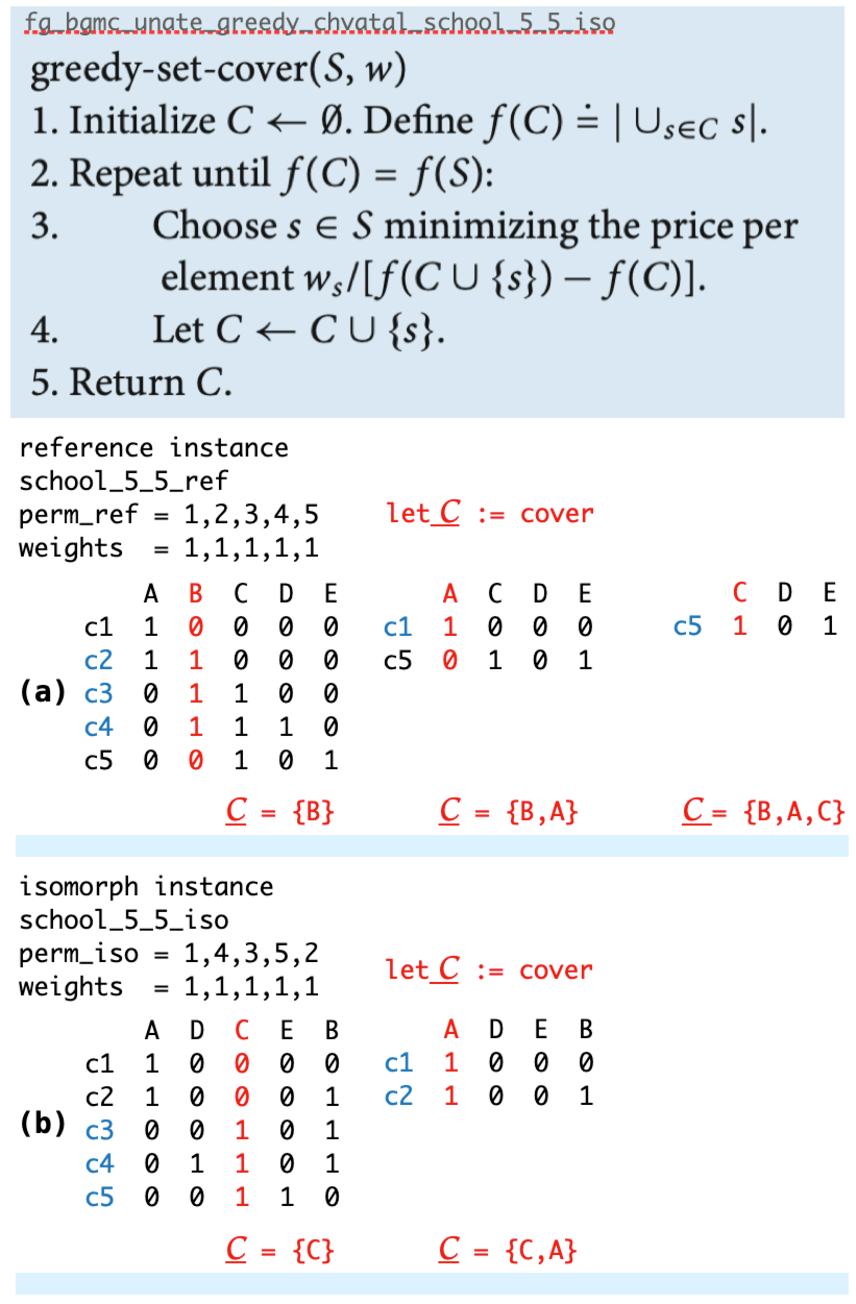
\includegraphics[width=0.45\textwidth]{_Figures/fg_bgmc_unate_greedy_chvatal_iso_school_5_5}
\caption{
The pseudo code of the greedy algorithm above is 
from~\cite{OPUS-setc-2016-Springer-Young-Greedy};
it represents the version of the Chvatal's algorithm 
in~\cite{OPUS-setc-1979-OR-Chvatal-greedy}.
The R-function that implements this algorithm is named
{\tt unate\_greedy\_chvatal\_basic} 
in Figure~\ref{fg_bgmc_unate_greedy_chvatal_stoc}a.
%
The algorithm is invoked on two instance bigraphs, represented
as two incidence matrices:
(a) the reference instance {\tt school\_5\_5\_ref}, and 
(b) the instance isomorph  {\tt school\_5\_5\_iso}.
As implied by the matrix structure, the weight of each column is 1.
For (a), the algorithm selects the 
{\it first column with minimum rate between column weight and column degree},
i.e. column B. In the next iteration, there remain only two rows to consider: s1 and s5. The first column with maximum degree is now column A. The algorithm terminates by selecting column C, returning a solution as 3 columns \{B, A, C\} and the total weight of 3.
%
For (b), the algorithm selects C as the first column with minimum rate between column weight and column degree. The next iteration is also the last. With the selection of
column A,  we get a solution as 2 columns \{C, A\} and the total weight of 2.
\vspace*{-4ex}
}
\label{fg_bgmc_unate_greedy_chvatal_iso_school_5_5}
\end{figure}


The isomorphs revisited in this article have a different context
and formulation. Their merits, to change the
{\it representation} of the problem without changing the problem itself,
have already been demonstrated
by solving instances of combinatorial problems. 
In the worst case,  solvers may timeout for some, but not all, isomorphs before finding the optimum solution 
\cite{
OPUS2-2001-BDD-STTT-Harlow,
OPUS2-2001-crossnum-JEA-Stallmann,
OPUS2-2005-sat-AMAI-Brglez,
OPUS2-2005-cover-DAC-Li,
OPUS2-2007-isomorph-ExpCS-Brglez}.
%
%
\par
The pseudo code of the greedy algorithm in 
Figure~\ref{fg_bgmc_unate_greedy_chvatal_iso_school_5_5},
is the core for our stochastic algorithm.
Two instance isomorphs illustrate the  
importance of  {\it representation}
when invoking the same greedy algorithm on each of the two
instances: we observe two solutions that differ by 50\%.
A narative that follows provides a simple interpretation
on how these two instances could have been created:
\begin{quote}
{\small
Scale down the bigraph instance in Figure~\ref{fg_bgmc_matching_cover}
and transform it to an incidence matrix with 5 columns and 5 rows.
The 5 columns represent 5 applicants
\{A, B, C, D, E\} who applied to teach one or more
of the 5 classes \{c1, c2, c3, c4, c5\}.
Two administrators are performing interviews with all applicants.
Administrator (a) interviews applicants in alphabetical order and marks
course qualifications for each applicant. 
%,  in natural order, in the incidence matrix (a): 
Applicant B, under the second column, is qualified to  teach classes \{c2, c3, c4\}.
Administrator (b) interviews applicants in a permuted order, \{A, D, C, E, B\}, and marks %,  in permuted order,
qualification for each applicant in the incidence matrix (b): 
marks about applicant B are now entered into the column 5.
}
\end{quote}

%%%%% EXPERIMENTS: chvatal_iso VERSUS chvatal_stock
%
%source("./__init_rBed_01.R")
%  rBedPath = glob[["rBedPath"]]  
%  glob[["workDir"]] = paste0(rBedPath, "/rBed_bgmc", "/workDir") 
%  source(paste0(rBedPath, "/_lib_R", "/__lib_R_resources.R"))
%  dataDir     = paste0(rBedPath, "/_data_tiny/bigraph/unate")
%  instanceDef = file.path(dataDir, "school_5_5__0.cnfU")
%  unate_greedy_chvatal_iso_experiment_distr(instanceDef, replicateSize=99)
%  
%instanceDef = school_5_5__0.cnfU 
%unate_greedy_chvatal_iso_experiment_distr(instanceDef, replicateSize=99)
%             replicateSize     = 99 
%             isSeedConsecutive = TRUE 
%                      date     = Sat Nov  6 12:15:37 2021 
%   ratio ratio_cnt
%1:   1.0        45
%2:   1.5        55
%
%instanceDef = school_5_5__1.cnfU 
%unate_greedy_chvatal_iso_experiment_distr(instanceDef, replicateSize=99)
%             replicateSize     = 99 
%             isSeedConsecutive = TRUE 
%                      date     = Sat Nov  6 12:15:21 2021 
%   ratio ratio_cnt
%1:   1.0        55
%2:   1.5        45
%
%instanceDef = school_5_5__0.cnfU 
%unate_greedy_chvatal_stoc_experiment_distr(instanceDef, replicateSize=99)
%             replicateSize     = 99 
%             isSeedConsecutive = TRUE 
%                      date     = Sat Nov  6 12:24:26 2021 
%   ratio ratio_cnt
%1:   1.0        45
%2:   1.5        55
%
%instanceDef = school_5_5__1.cnfU 
%unate_greedy_chvatal_stoc_experiment_distr(instanceDef, replicateSize=99)
%             replicateSize     = 99 
%             isSeedConsecutive = TRUE 
%                      date     = Sat Nov  6 12:26:58 2021 
%   ratio ratio_cnt
%1:   1.0        55
%2:   1.5        45

%instanceDef = school_9_11__0.cnfU 
%unate_greedy_chvatal_iso_experiment_distr(instanceDef, replicateSize=99)
%             replicateSize     = 99 
%             isSeedConsecutive = TRUE 
%                      date     = Sat Nov  6 12:30:21 2021
%   ratio ratio_cnt
%1:  1.00        27
%2:  1.25        52
%3:  1.50        21
%
%instanceDef = school_9_11__0.cnfU 
%unate_greedy_chvatal_stoc_experiment_distr(instanceDef, replicateSize=99)
%             replicateSize     = 99 
%             isSeedConsecutive = TRUE 
%                      date     = Sat Nov  6 12:32:31 2021 
%   ratio ratio_cnt
%1:  1.00        27
%2:  1.25        52
%3:  1.50        21
\par\noindent
The performance of  many greedy algorithms is measured as
a {\it ratio}:
\par\vspace*{-2ex}
\begin{equation}   \label{eq_ratio}
  {\it  ratio} := {\it  value\_greedy} / {\it  BKV}
\end{equation}
%\par\noindent\vspace*{-1.5ex}
%\noindent
where {\it value\_greedy} is returned by the greedy algorithm 
and {\it BKV} is the {\it best-known-value} (BKV),
associated with the given instance such as 
{\tt school\_5\_5\_ref}.
Ideally, BKV represents the
proven optimum solution with an ILP-like solver,
otherwise we use the best known published value. 
As expected for the  example above,
BKV = 2 for both {\tt school\_5\_5\_ref} and {\tt school\_5\_5\_iso}.

The complete R-code of the stochastic greedy algorithm 
that relies on invoking any number of instance isomorphs is
depicted in 
Figure~\ref{fg_bgmc_unate_greedy_chvatal_stoc}a.
Consistent with definition in Eq.~\ref{eq_ratio}, 
Table~\ref{tb_bgmc_unate_greedy_chvatal_school_5_5_iso}
reports a statistical summary of experiments that involve
100 isomorphs of {\tt school\_5\_5\_ref} and 
100 isomorphs of {\tt school\_5\_5\_iso}.
%
%
\begin{table}[h!]
\vspace*{-1.1ex} 

\caption{
% NO \par\noindent statements in captions under ieee-format
A statistical summary of results, based on  experiments that involve
100 isomorphs, initialized with 100 seeds, created from each of the two instances: 
{\tt school\_5\_5\_ref} and {\tt school\_5\_5\_iso}.
For the complete R-code of the stochastic greedy algorithm 
that relies on invoking any number of instance isomorphs, the algorithm
{\tt unate\_greedy\_chvatal\_iso} in
Figure~\ref{fg_bgmc_unate_greedy_chvatal_stoc}a.
However, identical results can also be generated,
using the same seeds,
with the alternative algorithm 
{\tt unate\_greedy\_chvatal\_stoc} in
Figure~\ref{fg_bgmc_unate_greedy_chvatal_stoc}b.
%\vspace{-2.15ex}
}
\hspace*{0.5em}
\vspace*{-1ex}
\begin{minipage}{0.40\textwidth}
\begin{Verbatim}[frame=lines, fontsize=\footnotesize,numbers=left,
numbersep=3pt,firstline=1,xleftmargin=9mm]
instanceDef = school_5_5_ref.cnfU 
unate_greedy_chvatal_iso_experiment_distr(
                              instanceDef)
                                                            
num_seeds =    100 ;    1,000  ;    10,000
  ratio  ratio_cnt ; ratio_cnt ; ratio_cnt
    1.0         45        541         5013
    1.5         55        459         4987
%
instanceDef = school_5_5_iso.cnfU 
unate_greedy_chvatal_iso_experiment_distr(
                              instanceDef)
                                                            
num_seeds =    100 ;    1,000  ;    10,000
  ratio  ratio_cnt ; ratio_cnt ; ratio_cnt
    1.0         55        459         4987
    1.5         45        541         5013
\end{Verbatim}
\end{minipage}

\label{fg_gray_02_coupon_6_markov}
\end{table}
%
\par
The main conclusion of the experiment in 
Table~\ref{tb_bgmc_unate_greedy_chvatal_school_5_5_iso} is this:
for both isomorph classes, with increasing number of seeds
\{100, 1,000, 10,000\} for
{\tt school\_5\_5\_ref} and {\tt school\_5\_5\_iso},
the probabilities of the best-case {\tt ratio} = 1.0 
and the worst-case {\tt ratio} = 1.5,  
converge to 0.50\%. This results is specific for the
instances which are isomorphs themselves. 
For a divers distribution of
{\tt ratio} spreads, see the results in
Figure~\ref{fg_bgmc_unate_greedy_chvatal_stoc_distr}
and
Table~\ref{tb_bgmc_data}.
 
Related to the worst-case ratio reported by the greedy algorithm
is the upper bound {\it UB} on the maximum value that could be
returned by the greedy algorithm. 
The search for  `tight'  upper bounds 
is still ongoing,
e.g.~\cite{
OPUS-setc-2012-LBCS-Saket-UB,
OPUS-setc-2016-OR-Felici-UB,
OPUS-setc-2019-STOC-Abboud-UB}.
%
%OPUS-setc-2012-LBCS-Saket-UB
%https://link.springer.com/chapter/10.1007/978-3-642-32512-0_25
%New and Improved Bounds for the Minimum Set Cover Problem
%Cite this paper as:
%Saket R., Sviridenko M. (2012) New and Improved Bounds for the Minimum Set Cover Problem. In: Gupta A., Jansen K., Rolim J., Servedio R. (eds) Approximation, Randomization, and Combinatorial Optimization. Algorithms and Techniques. APPROX 2012, RANDOM 2012. Lecture Notes in Computer Science, vol 7408. Springer, Berlin, Heidelberg. https://doi.org/10.1007/978-3-642-32512-0_25
%
%OPUS-setc-2016-OR-Felici-UB
%https://www.semanticscholar.org/paper/A-priori-upper-bounds-for-the-set-covering-problem-Felici-Ndreca/2fdb29f627f29d563988b60bac9cbde5e21f6a22
%@article{OPUS-setc-2016-,
%  title={A-priori upper bounds for the set covering problem},
%  author={Giovanni Felici and Sokol Ndreca and Aldo Procacci and Benedetto Scoppola},
%  journal={Annals of Operations Research},
%  year={2016},
%  volume={238},
%  pages={229-241}
%}
% 
%OPUS-setc-2019-STOC-Abboud,-UB
%Dynamic set cover: improved algorithms and lower bounds
%https://dl.acm.org/doi/10.1145/3313276.3316376
% 
However, not one of these publications offers
{\em empirical evidence} of how tight these bounds really are
for {\em any} specific instances
relatively to Chvatal's bound in~\cite{OPUS-setc-1979-OR-Chvatal-greedy}.
The upper bound UB we use in 
this article has been formulated in~\cite{OPUS-setc-1979-OR-Chvatal-greedy}.
For an illustration of how we apply this bound to instances in this article,
see Figure~\ref{fg_bgmc_unate_greedy_chvatal_UB}.
%
\begin{figure}[t!]
\vspace*{-2ex}
\centering
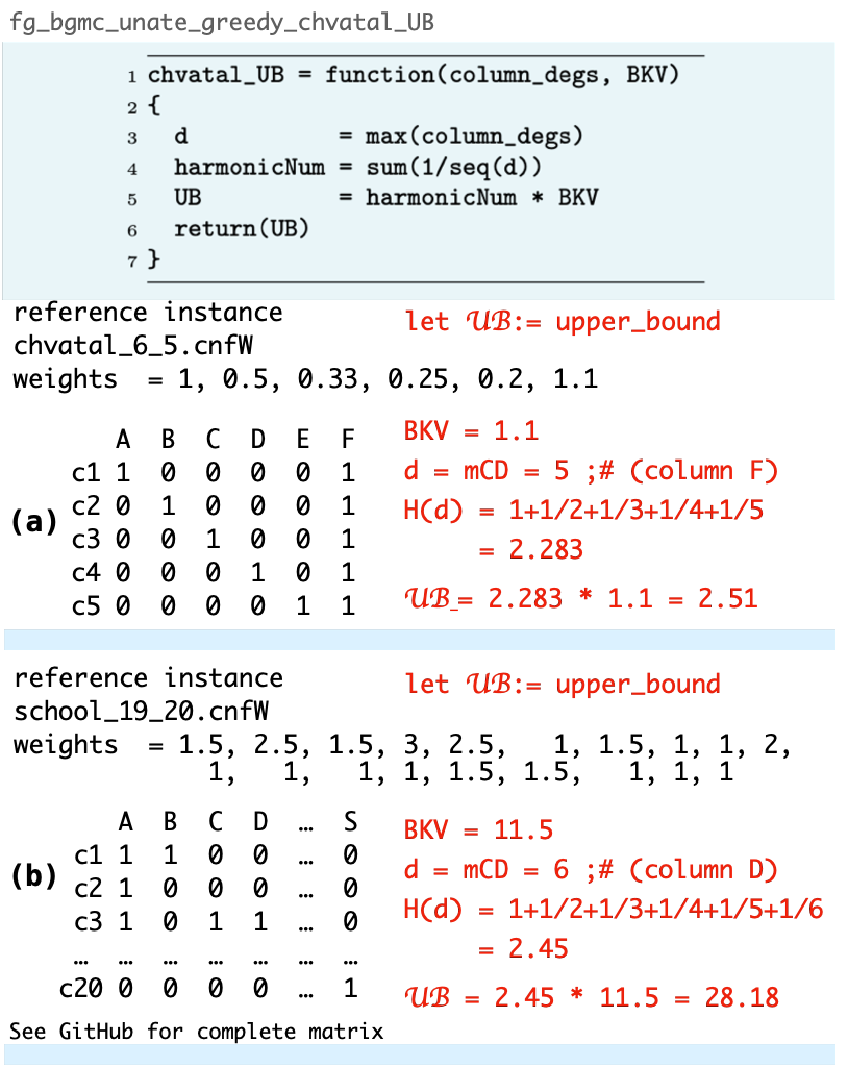
\includegraphics[width=0.45\textwidth]{_Figures/fg_bgmc_unate_greedy_chvatal_UB}
\caption{
Two examples of computing the minimum set cover upper bound UB.
The first instance is a test case introduced 
in~\cite{OPUS-setc-1979-OR-Chvatal-greedy}.
\vspace*{-2.5ex}
}
\label{fg_bgmc_unate_greedy_chvatal_UB}
\end{figure}
 


The next section 
introduces a simplification of the greedy algorithm, 
replacing the isomorph-based solver  
{\tt unate\_greedy\_chvatal\_iso}
with an alternative solver,
{\tt unate\_greedy\_chvatal\_stoc}.
%  return(c(coordBest, valueBest, agentId, 
%           steps, probes, isCensored))

%  return(c(coordBest, valueBest, agentId, 
%           steps, probes, isCensored))
\begin{figure*}[t!]
\vspace*{-9ex} 
\hspace*{-2.1em}
\begin{minipage}{0.51\textwidth}
\centering

{\large\bf  (a) }
\vspace*{-1ex} 
\begin{Verbatim}[frame=lines, fontsize=\footnotesize,numbers=left,
numbersep=3pt,firstline=1,xleftmargin=9mm]
unate_greedy_chvatal_basic = function() 
{
  # required inputs
  n           = glob[["nCols"]]
  m           = glob[["mRows"]]
  M           = glob[["M_ref"]]
  colWeights  = glob[["colWeights_ref"]]  
  # local initializations
  nOps        = 0
  coord       = rep(0, n)
  
  while(TRUE) {
    percentages = colWeights / colSums(M) 
    if (all(percentages == Inf)) { break }
    jdx         = which.min(percentages)
    rem_vec     = which(M[,jdx] %in% 1)
    M[rem_vec,] = 0
    coord[jdx]  = 1
    nOps        = nOps + 1
  }
  coordGreedy = paste(coord, collapse = "")
  valueGreedy = as.numeric(t(coord) %*% colWeights))
  
  return(list(
    coordGreedy = coordGreedy, 
    valueGreedy = valueGreedy,
    nOps        = nOps))
} 
\end{Verbatim}
\vspace*{-6.5ex}
\begin{Verbatim}[frame=lines, fontsize=\footnotesize,numbers=left,
numbersep=3pt,firstline=1,xleftmargin=9mm]
unate_greedy_chvatal_iso = function(replicaId=0) 
{  
  # required inputs 
  n               = glob[["nCols"]]
  m               = glob[["mRows"]]
  M_ref           = glob[["M_ref"]]
  colWeights_ref  = glob[["colWeights_ref"]]
  greedyId        = glob[["greedyId"]]   
  if (replicaId == 0) {
    coordPermV = 1:n # reference permutation (natural order)
    coordPerm  = paste(coordPermV, collapse=",")
    colWeights = glob[["colWeights_ref"]] 
    M          = glob[["M_ref"]]
 
  } else {
    # create an isomorph instance, controlled by replicaId
    set.seed(replicaId)
    coordPermV = sample(1:n)
    coordPerm  = paste(coordPermV, collapse=",")
    colWeights = c()
    M          = matrix(rep(NA, m*n), ncol=n)
    for (idx in 1:n) {
      i = idx
      j = coordPermV[idx] 
      colWeights[idx] = glob[["colWeights_ref"]][j]
      M[ ,idx]        = glob[["M_ref"]][,j]
    }
  }
  # invoke unate_greedy_chvatal_basic() with new variables 
  glob[["M_ref"]]          = M
  glob[["colWeights_ref"]] = colWeights
  glob[["replicaId"]]      = replicaId 
  answ = unate_greedy_chvatal_basic()
  
  coordGreedy = answ$coordGreedy
  valueGreedy = answ$valueGreedy ; nOps = answ$nOps
  return(list(coordGreedy=coordGreedy, 
              valueGreedy=valueGreedy, nOps=nOps))
 }
  \end{Verbatim}
\end{minipage}
%
\begin{minipage}{0.51\textwidth}
\centering
%\vspace*{-1ex}

{\large\bf  (b) }
\vspace*{-1ex} 
\begin{Verbatim}[frame=lines, fontsize=\footnotesize,numbers=left,
numbersep=3pt,firstline=1,xleftmargin=9mm]
unate_greedy_chvatal_stoc = function() 
{
  # required inputs
  M          = glob[["M_ref"]]
  n          = glob[["nCols"]]
  m          = glob[["mRows"]]
  colWeights = glob[["colWeights_ref"]]
  replicaId  = glob[["replicaId"]]
  # local initializations
  nOps       = 0
  coord      = rep(0, n)
  
  while(TRUE) {
    percentages = colWeights / colSums(M)
    if (all(percentages==Inf)) { break }
    if (replicaId == 0) {
      jdx     = which.min(percentages)
    } else {
      jdx_vec = which(percentages == min(percentages))
      jdx_cnt = sample(1:length(jdx_vec))[1]
      jdx     = jdx_vec[jdx_cnt]         
    }
    rem_vec     = which(M[,jdx] %in% 1)
    M[rem_vec,] = 0
    coord[jdx]  = 1
    nOps        = nOps + 1
  }
  
  coordGreedy = paste(coord, collapse = "")
  valueGreedy = as.numeric(t(coord) %*% colWeights))
  
  return(list(
    coordGreedy = coordGreedy, 
    valueGreedy = valueGreedy,
    nOps        = nOps))
}
\end{Verbatim}
\vspace*{-6.5ex}
\begin{Verbatim}[frame=lines, fontsize=\footnotesize,numbers=left,
numbersep=3pt,firstline=1,xleftmargin=9mm]
unate_greedy_chvatal_stoc_experiments = 
  function(instanceDef, isSeedConsecutive=T, replicateSize=10) {
  
  # read instance file and convert to matrix with detailed info
  # data store in global list, glob
  
  read_bgu(instanceDef)
  dt = data.table()
  for (replicaId in 0:replicateSize) {
    
    glob[["replicaId"]] = replicaId
    if (isSeedConsecutive) {
      seedInit = replicaId 
    } else {
      seedInit = trunc(1e6*runif(1)) 
    }
    set.seed(seedInit)
    
    answ = unate_greedy_chvatal_stoc() 
    coordGreedy = answ$coordGreedy
    valueGreedy = answ$valueGreedy ; nOps = answ$nOps
    dt = rbind(dt, list(
      replicaId   = replicaId,
      nOps        = nOps,
      coordGreedy = coordGreedy,
      valueGreedy = valueGreedy
    ))
  }
  return(dt)
  
}
\end{Verbatim}


%\VerbatimInput[fontshape=sl,fontsize=\scriptsize,numbers=left,
%    numbersep=3pt,firstline=1,xleftmargin=3mm]{Figures/fg_markov.fpt.methods-R-txt}
\end{minipage}
\vspace*{2ex}
\caption{
% NO \par\noindent statements in captions under ieee-format
Two equivalent {\it stochastic versions} in R of the Chvatal's algorithm:   
(a) inducing distributions of set covers with bigraph isomorphs and
(b) inducing distributions of set covers by randomizing best selections. To achieve the randomization, when ${\rm replicaId} > 0$, we use the random selection returned by the R-function "which".
}
\label{fg_bgmc_unate_greedy_chvatal_stoc}
\end{figure*}



%
\subsection{{\sf On Set Covers with a Stochastic Greedy Algorithm}}
\noindent
The simplified stochastic greedy algorithm, 
replacing the isomorph-based implementation,
%{\tt unate\_greedy\_chvatal\_iso}
is represented by the function
{\tt unate\_greedy\_chvatal\_stoc} 
in Figure~\ref{fg_bgmc_unate_greedy_chvatal_stoc}b.
The distributions of set cover solutions are induced,
for ${\rm replicaId} > 0$, 
%{\em randomizing best selections},
by relying on the randomized selections returned by the R-function "which".

How can we claim that the very different implementations 
of the two greedy stochastic algoritms in 
Figures~\ref{fg_bgmc_unate_greedy_chvatal_stoc}a and 
\ref{fg_bgmc_unate_greedy_chvatal_stoc}b are equivalent?
In Figures~\ref{fg_bgmc_unate_greedy_chvatal_stoc}a 
we induce randomization by explicitly interchanging rows
in the matrix.
In Figures~\ref{fg_bgmc_unate_greedy_chvatal_stoc}b
we induce randomization by a random selection of columns 
with the same minimum rate between column weight and column degree.

Experiments have demonstrated, for {\em both solvers}, 
the same or close to the same distributions
of ratios such as shown in 
Table~\ref{tb_bgmc_unate_greedy_chvatal_school_5_5_iso},
and
Figure~\ref{fg_bgmc_unate_greedy_chvatal_stoc_distr}.
However, the runtime of 
{\tt unate\_greedy\_chvatal\_stoc} solver that relies on changing the seed
has better  runtime and easier interpretation than
{\tt unate\_greedy\_chvatal\_iso} solver that
relies on explicit permutations of matrix columns.
For specific isomorphs of interest, 
we do invoke a column permutation of
the respective reference instance such as
the example of instance {\tt school\_5\_5\_ref}.
%
%
\subsection{{\sf Runtime Experiments}}
\noindent
The runtime experiments with the minimum set cover instances are summarized in
Figure~\ref{fg_bgmc_unate_greedy_chvatal_stoc_distr},
Table~\ref{tb_bgmc_data}, 
Table~\ref{tb_bgmc_school_19_20}, and
Table~\ref{tb_bgmc_data_BRKGA}.

\begin{figure*}[t!]
\vspace*{-4ex}
\centering

{\sf (school\_9\_11.cnfU)} 
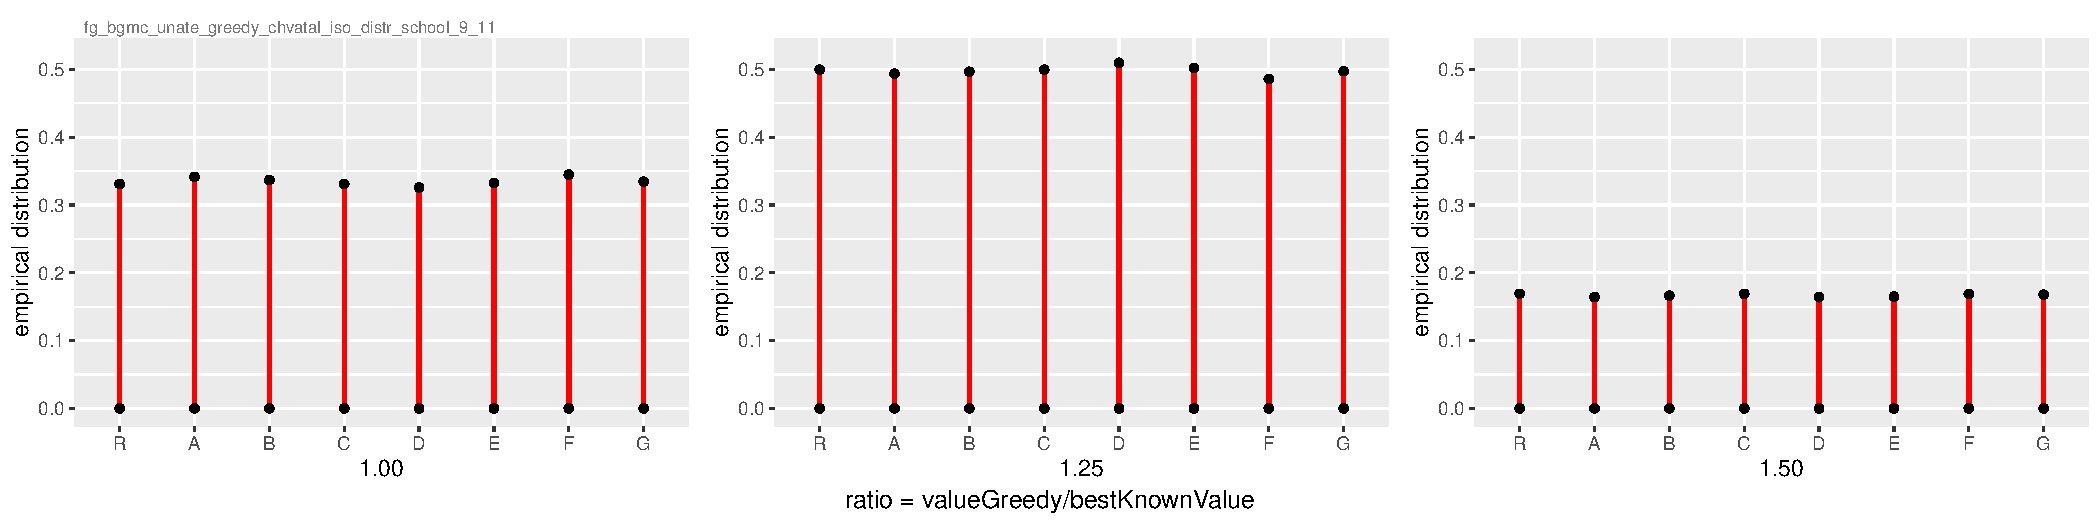
\includegraphics[width=0.90\textwidth]{_Figures/fg_bgmc_unate_greedy_chvatal_stoc_distr_school_9_11}
\\[2ex]
{\sf (ab)}\\
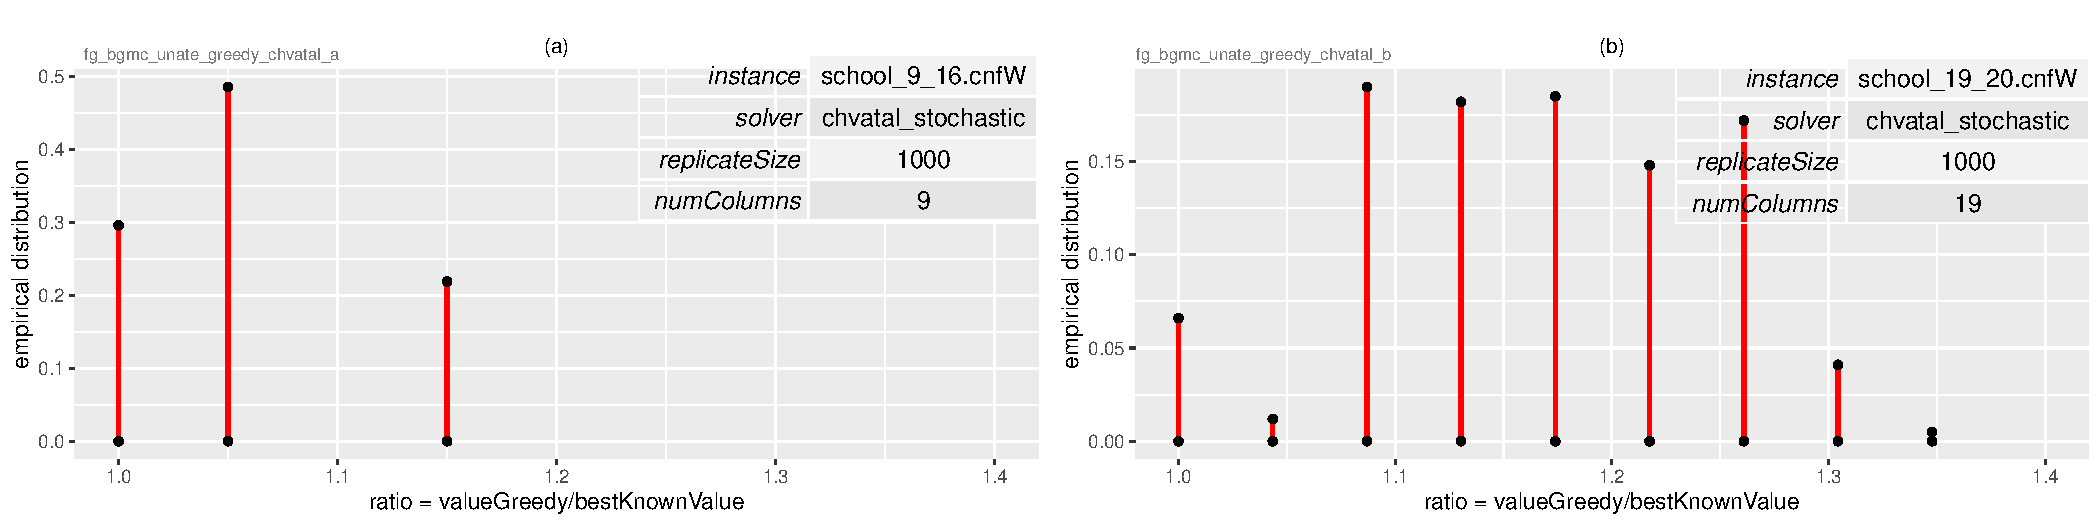
\includegraphics[width=0.90\textwidth]{_Figures/fg_bgmc_unate_greedy_chvatal_stoc_distr_ab}
\\[2ex]
{\sf (cd)}\\
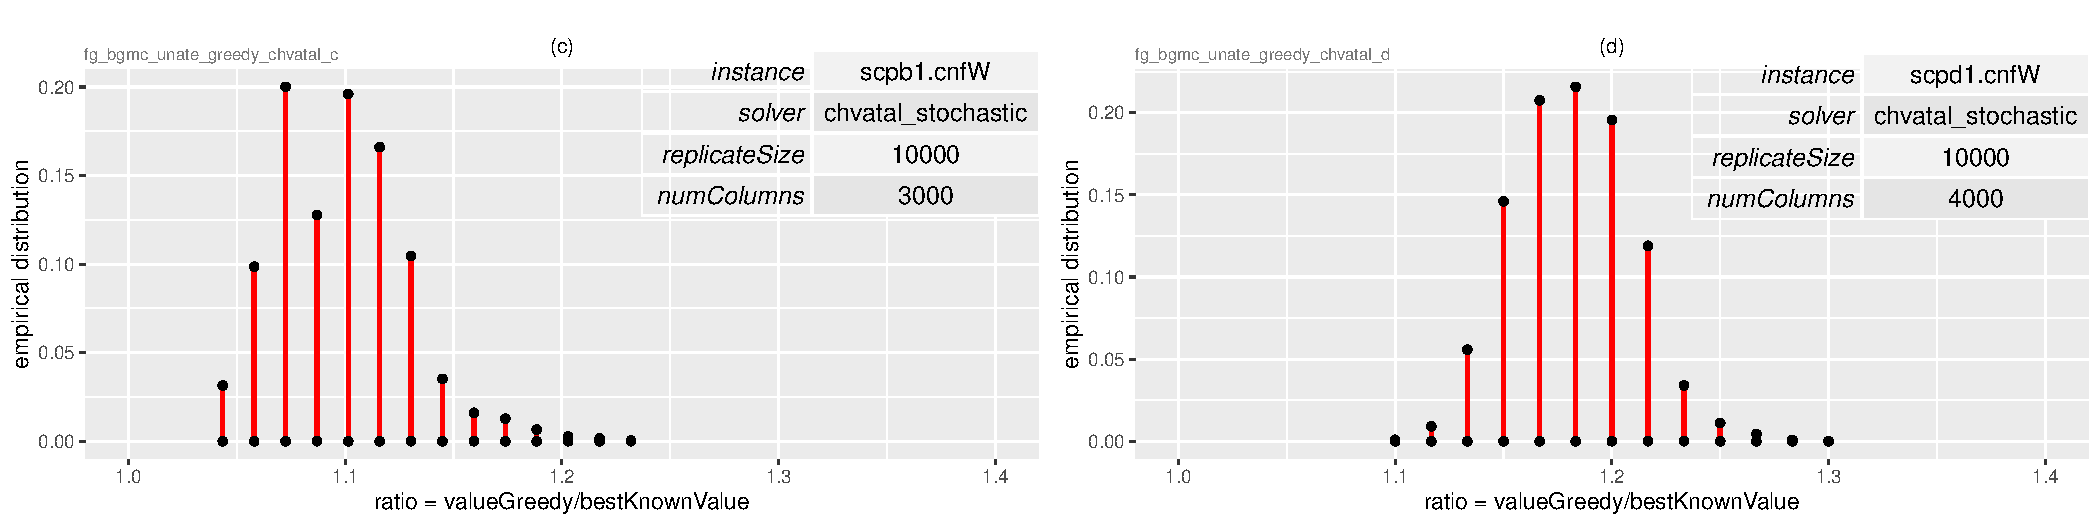
\includegraphics[width=0.90\textwidth]{_Figures/fg_bgmc_unate_greedy_chvatal_stoc_distr_cd}

\caption{
Reference parameters for each instance in this figure
are listed in Table~\ref{tb_bgmc_data}.
The top segment {\sf (school\_9\_11.cnfU)}
depicts  the empirical distribution of ratios \{1.0, 1.25, 1.5\}
for the 8 isomorph classes of size 10,000 each, induced by
the instance {\tt school\_9\_11.cnfU}. %
The middle segment {\sf (ab)}
depicts  distribution of ratios  
for two isomorph classes, each of size 1,000.
%
The bottom segment {\sf (cd)}
depicts  distribution of ratios the 
for two isomorph classes, each of size 10,000.
%
For additional details, see the article.
\vspace*{-3ex}
}
\label{fg_bgmc_unate_greedy_chvatal_stoc_distr}
\end{figure*}

\begin{description}

\item[\sf{Figure~\ref{fg_bgmc_unate_greedy_chvatal_stoc_distr}}]~\\\
The top segment {\sf (school\_9\_11.cnfU)}
depicts  the empirical distribution of ratios \{1.0, 1.25, 1.5\}
for the 8 isomorph classes of the instance {\tt school\_9\_11.cnfU}.
%extends the two ratio summary \{1.0, 1.5\} in
%Table~\ref{tb_bgmc_unate_greedy_chvatal_school_5_5_iso} 
This instance, % {\tt school\_9\_11},
already introduced in Figure~\ref{fg_bgmc_matching_cover},
induces isomorph classes \{{\sf R, A, B, C, D, E, D,F, G}\}.
The {\it reference class} {\sf R} represents 10,000 instance isomorphs of 
{\tt school\_9\_11\_R} = {\tt school\_9\_11}.
The {\it alternative class} {\sf A} represents 10,000 instance isomorphs of 
{\tt school\_9\_11\_A} = (seed-specific isomorph of {\tt school\_9\_11}).
The remainder of classes, \{B,...,G\}, are formed similarly.
%
The empirical distribution probabilities associated with each ratio
of the reference isomorph class {\sf R} of size 10,000 are itemized below:  
\par\vspace*{1.2ex}
\hspace*{1.6em}
\begin{minipage}{0.33\textwidth}
%\centering
\begin{Verbatim}[frame=lines, fontsize=\footnotesize,numbers=left,
numbersep=3pt,firstline=1,xleftmargin=9mm] 
   ratio ratio_cnt empirical_distr
1:  1.00      3311          0.3311
2:  1.25      4998          0.4998
3:  1.50      1691          0.1691
\end{Verbatim}
\end{minipage}

\par\vspace*{1.2ex}\noindent
As shown in the plot, empirical distributions of ratios of the
isomorph in classes from  \{A,...,G\}
closely match the 
reference isomorph class {\sf R}.
However, the variance between the isomorph classes
becomes noticeable with decreasing the
class size from 10,000 to 1,000 and 100 
-- just as already observed in
Table~\ref{tb_bgmc_unate_greedy_chvatal_school_5_5_iso}.

The middle segment labeled as {\sf (ab)}
depicts  distribution of ratios  
for two isomorph classes, each of size 1,000:
weight-specific {\tt school\_9\_16.cnfW} and 
weight-specific {\tt school\_19\_20.cnfW}.
For  the {\tt school\_9\_16.cnfW} isomorph class, 
we observe 3 distinct ratios in the range  \{1.0, 1.15\}.
For the {\tt school\_19\_20.cnfW} isomorph class,
we observe  9 distinct ratios in the range  \{1.0, 1.35\}.

The bottom segment of this figure, labeled as {\sf (cd)}
depicts  the empirical distribution of ratios  
for two isomorph classes, each of size 10,000:
weight-specific {\tt scpb1.cnfW} and 
weight-specific {\tt scpd1.cnfW}.
For the {\tt scpb1.cnfW} isomorph class,
we observe  14 distinct ratios in the range \{1.04, 1.23\}.
For the {\tt scpd1.cnfW} isomorph  class,
we observe  13 distinct ratios in the range \{1.10, 1.30\}.

\item[\sf{Table~\ref{tb_bgmc_data}}]~\\\
%The Table~\ref{tb_bgmc_data} 
This table
introduces all instances
that summarize results of experiments in this article.
Details about instance parameters have been discussed
in Section~\ref{sec_matching} when introducing
the maximum matching solvers.
Additional columns in this table, relevant to
the minimum set cover solvers  
in this section include
{\it BKV, UB, value\_Chvatal\_stats, and BKV\_ratio\_stats}.
The definition of {\it ratio} in Equation~\ref{eq_ratio}
relies on the {\it best-known-value} {\it BKV}. 
The computation of the Chvatal's upper bound 
{\it UB} on the minimum set cover is illustrated in
Figure~\ref{fg_bgmc_unate_greedy_chvatal_UB}.
The column {\it value\_Chvatal\_stats} reports the 
empirical set cover statistics with solver {\tt unate\_greedy\_chvatal\_stoc},
the stochastic version of the Chvatal's greedy algorithm.
The reported statistics represents comma-separated
values of minimum, median, mean, standard deviation, and maximum.
The column {\it  BKV\_ratio\_stats} reports
the same statistics, normalized with respect to {\it BKV}.

There are 37 instances in Table~\ref{tb_bgmc_data}.
The question arises of how effective 
the stochastic greedy algorithm solver
{\tt unate\_greedy\_chvatal\_stoc} 
actually is.
A partial glimpse is shown in the table below:

\par\vspace*{1.2ex}
\hspace*{0.8em}
\begin{minipage}{0.36\textwidth}
\begin{Verbatim}[frame=lines, fontsize=\footnotesize,numbers=left,
numbersep=3pt,firstline=1,xleftmargin=9mm]      
    ranges_of_ratios  counts_out_of_37     
        ratio  = 1.0                12                
1.00 <  ratio <= 1.1                18                
1.20 <= ratio <= 2.5                 7                 
\end{Verbatim}
\end{minipage}
\par\vspace*{1.1ex}\noindent
The counts about in the table above signify:
\begin{itemize}
\item
optimum solutions have been found for 12-out-37 instances, 
\item
solutions within 10\% of the optimium have been found for 18-out-37 instances,
\item
solutions above 20\% of the optimium have been found for 7-out-37 instances.
\end{itemize}

\begin{table*}[h!]
\vspace*{1.9ex} 
\caption{
Similar size instances and their variabilities: BKVs, UBs, Chvatal ratios, and harmonic numbers.
For  details, see the article.
}
\label{tb_bgmc_school_19_20}
\hspace*{2.8em}
% \begin{center}
\begin{minipage}{0.85\textwidth}
%\centering
\begin{Verbatim}[frame=lines, fontsize=\footnotesize,numbers=left,
numbersep=3pt,firstline=1,xleftmargin=9mm] 
                                    exact                                chvatal  chvatal  
                                    column_solutions/                    best     worst   harmonic  
instance             weight_range   column_degrees        BKV      UB    ratio    ratio     number  
school_19_20.cnfU    [1.0,   1.0]   2,4,5,6,15,16/         6      14.7    1.0      1.0      2.45
                                    5,6,5,1, 3, 3
school_19_20.cnfW    [1.0,   3.0]   1,5,7,9,10,14,17,18/  11.5    28.18   1.0      1.348    2.45      
                                    3,5,3,2, 4, 2, 2, 2
school_19_20_1.cnfW  [0.333, 1.0]   1,5,7,9,10,14,17,18/   3.833   9.39   1.087    1.304    2.45
                                    3,5,3,2, 4, 2, 2, 2    
school_19_20_5.cnfW  [0.7,   4.9]   1,4,5,7,9,15,16/      16.1    39.45   1.087    1.087    2.45
                                    3,6,5,3,2  3, 3           
chvatal_19_18.cnfW   [0.33,  1.1]   19/                    0.5     1.75   1.0      1.0      3.496 
                                    18                            
\end{Verbatim}
\end{minipage}
%column_j     "1,2,3,4,5,6,7,8,9,10,11,12,13,14,15,16,17,18,19"
%column_degs  "3,5,3,6,5,1,3,2,2, 4, 2, 2, 2, 2, 3, 3, 2, 2, 2"
%column_sols  "  2,  4,5,6,                     15,16"
%column_degs  "  5,  6,5,1,                      3, 3"
%column_sols  "  2,4,5,6,15,16"
%column_degs  "  5,6,5,1, 3, 3"
%
%column_j     1,2,3,4,5,6,7,8,9,10,11,12,13,14,15,16,17,18,19
%column_degs  3,5,3,6,5,1,3,2,2, 4, 2, 2, 2, 2, 3, 3, 2, 2, 2
%column_sols  1,5,        7,  9,10,         14,      17,18  
%column_degs  3,      5,  3,  2, 4,          2,       2, 2     
%
%column_j     1,2,3,4,5,6,7,8,9,10,11,12,13,14,15,16,17,18,19
%column_degs  3,5,3,6,5,1,3,2,2, 4, 2, 2, 2, 2, 3, 3, 2, 2, 2
%column_sols  1,      5,  7,  9,10,         14,      17,18  
%column_degs  3,      5,  3,  2, 4,          2,       2, 2   
%
%column_j     1,2,3,4,5,6,7,8,9,10,11,12,13,14,15,16,17,18,19
%column_degs  3,5,3,6,5,1,3,2,2, 4, 2, 2, 2, 2, 3, 3, 2, 2, 2
%column_sols  1,5,        7,  9,10,         14,      17,18  
%column_degs  3,      5,  3,  2, 4,          2,       2, 2     
%
%column_j     1,2,3,4,5,6,7,8,9,10,11,12,13,14,15,16,17,18,19
%column_degs  3,5,3,6,5,1,3,2,2, 4, 2, 2, 2, 2, 3, 3, 2, 2, 2
%column_sols  1,    4,5,  7,  9,               15,16  
%column_degs  3,    6,5,  3,  2                 3, 3    
\vspace*{-2.5ex}
\end{table*}  

\item[\sf{Table~\ref{tb_bgmc_school_19_20}}]~\\\
This table assembles four versions of 19-column, 20-row instance 
{\tt school\_19\_20}: one with {\it all weights at 1}, and three with
weights in the ranges shown.
The fifth instance, {\tt chvatal\_19\_18}, is
a scaled-up instance of {\tt chvatal\_6\_5} introduced 
in~\cite{OPUS-setc-1979-OR-Chvatal-greedy}.
In {\tt chvatal\_6\_5}, only the weight of the column 6
determines its BKV.  In {\tt chvatal\_19\_18},
BKV = 0.5 for the solution column 19 and weight = 0.5.
For more observations, see below:
\begin{itemize}
\item
As already demonstrated in Table~\ref{tb_bgmc_data},
the ratios UB/BKV $>$ 2, i.e. UB is not a tight upper bound. 
Weight range %variability 
impacts UB significantly.
\item
Weight range also impacts significantly 
the minimum and the maximum range of ratio 
returned by the solver {\tt unate\_greedy\_chvatal\_stoc}.
The harmonic number is determined by
{\tt max(column\_degrees)} only.
The ratio {\tt harmonic\_number/worst\_ratio)} 
varies from 2.35/1.348 = 1.743 to 3.496.
\end{itemize}


\begin{table*}[h!]
\vspace*{2.5ex} 
\caption{
This is an extension of~Table~\ref{tb_bgmc_data}.
The {rows~3--5} refer to three large instances from the 
OR-library~\cite{OPUS-setc-2014-orlib-Beasley}.
The {rows~6--8} introduce {\it almost identical} instances
related to instances on rows  {rows~3--5} with the exception that now 
{\it all weights are set to 1.}
For %additional 
details, see the article.
%\vspace{-4.05ex}
%
%{\tt BRKGA}~\cite{OPUS-setc-2014-BRKGA-Resende-code}. 
%there no better BKVs in the li
%
%o three large instances from the 
%OR-library~\cite{OPUS-setc-2014-orlib-Beasley}.
%Experiments with these instances
%verify the nominal performance of the 
%\CPP solver {\tt BRKGA}~\cite{OPUS-setc-2014-BRKGA-Resende-code}. 
%The best-known-values (BKVs)
%returned by this solver match the BKVs reported 
%elsewhere~\cite{OPUS-setc-2014-SWJ-Broderick-Bee_Colony}:
%\{69, 227, 60\}. 
%compare BKV to {\tt best\_cover} values returned by
%solvers {\tt unate\_greedy\_chvatal\_stoc} and {\tt BRKGA}
%and also 
%the runtimes of 
%solvers {\tt unate\_greedy\_chvatal\_stoc} and {\tt BRKGA}
%under the limits of 10,000 seeds ({\tt num\_seeds})
%and 200 generations ({\tt num\_gens}).
%
%The rows~6--8 compare BKV runtimes of 
%solvers {\tt unate\_greedy\_chvatal\_stoc} and {\tt BRKGA}
%under the limits of 10,000 seeds ({\tt num\_seeds})
%and 200 generations ({\tt num\_gens}).
%Experiments with instances on rows 3--5
%
%%
%However, instances on  rows 6--8, where all weights are set to 1,
%the minimum set cover problem becomes significantly more difficult.
%Under comparable computational cost ({\tt num\_gens = 200}), 
%the \CPP~solver {\tt BRKGA} returns best cover values 
%as~\{25, 47, 27\}
%whereas the \R~solver {\tt unate\_greedy\_chvatal\_stoc}
%returns significantly better cover values 
%of~\{22, 44, 25\} -- 
%at much lower computational cost!
}
\hspace*{6.0em}
\begin{minipage}{0.73\textwidth}
\begin{Verbatim}[frame=lines, fontsize=\footnotesize,numbers=left,
numbersep=3pt,firstline=1,xleftmargin=9mm] 
                     chvatal         BRKGA      chvatal  chvatal     BRKGA    BRKGA
  instance   BKV  cover_best    cover_best    num_seeds  seconds  num_gens  seconds 
scpb1.cnfW    69          72            69       10,000    1,271       200    2,505 
scpc1.cnfW   227         249           227       10,000    2,601       200    5,274    
scpd1.cnfW    60          66            60       10,000    1,666       200    5,377  
scpb1.cnfU    22          22            25       10,000      838       200    3,078     
scpc1.cnfU    44          44            47       10,000    1,444       200    4,764   
scpd1.cnfU    25          25            27       10,000    1,120       200    5,713           
\end{Verbatim}
\end{minipage}
% \end{center}
\label{tb_bgmc_data_BRKGA}
\vspace*{2ex}
\end{table*}

\item[\sf{Table~\ref{tb_bgmc_data_BRKGA}}]~\\\
This table supplements the results of 
the greedy set cover experiments summarized in Table~\ref{tb_bgmc_data}.
The six instances from 
Table~\ref{tb_bgmc_data} 
summarize the most important results obtained to date with
the solver {\tt unate\_greedy\_chvatal\_stoc},
running each instance with 10,000 unique seeds,
equivalent to processing 10,000  isomorphs 
of each of six instances.
\begin{itemize}
\item
The {rows~3--5} refer to three large instances from the 
OR-library~\cite{OPUS-setc-2014-orlib-Beasley}.
Experiments with these instances
verify the nominal performance of the 
\CPP~solver 
{\tt BRKGA}~\cite{
  OPUS-setc-2014-BRKGA-Resende-code,
  OPUS-setc-2014-BRKGA-Resende} 
reporting the minimum cover value found after running each instance 
with the {\it generation limit} of 200.
The best covers
returned by this solver match the BKVs reported 
elsewhere~\cite{OPUS-setc-2014-SWJ-Broderick-Bee_Colony}:
\{69, 227, 60\}. These covers dominate 
the best covers returned by
{\tt unate\_greedy\_chvatal\_stoc}: 
\{72, 249, 66\}.
\item
The {rows~6--8} introduce {\it almost identical} instances
related to instances on rows  {rows~3--5} with the exception that now 
{\it all weights are set to 1.}
There are no better covers 
than the ones reported by 
\R~solver {\tt unate\_greedy\_chvatal\_stoc} in this article:
\{22, 44, 25\}. The best covers 
returned by  \CPP~solver {\tt BRKGA} are significantly worse:
\{25, 47, 27\}. 
%Hence we designate \{22, 44, 25\} the best-known-covers these new instances.
\end{itemize}

The results on lines 6--8 in Table~\ref{tb_bgmc_data_BRKGA} 
are new: they provide the currently {\it best-known-values} (BKVs) for the
three largest OR-instances listed on lines 6--8. 
This may well be the first time where a greedy algorithm outperforms
a state-of-the-art algorithm designed to search for optimum solutions -- 
not only in runtime but more importantly, in delivering 
significantly better solutions.
\end{description}

%Nunc eleifend consequat lorem. Sed lacinia nulla vitae enim. Pellentesque tin- cidunt purus vel magna. Integer non enim. Praesent euismod nunc eu purus. Donec bibendum quam in tellus. Nullam cursus pulvinar lectus. Donec et mi. Nam vulputate metus eu enim. Vestibulum pellentesque felis eu massa. 
